\documentclass[notitlepage]{article}
\usepackage{amsmath, amssymb}
\usepackage{enumerate}
\usepackage[margin=1in]{geometry}
\usepackage{tikz}
\usepackage{standalone}
\usepackage{graphicx}
\usepackage{subfig}
\usepackage{cases}

\setlength\parindent{0pt}

\begin{document}
Author: Jacky Leung

This is a concise, cheat-sheet-style set of notes for ECON 3143: Macroeconomic Theory II at HKUST. The primary focus is on the mathematical derivation of models, though key economic intuitions are also highlighted. Graphical examples, such as the movements of curves, are largely omitted for brevity. Content is based on Professor Jenny Xu's lecture notes and course materials, and the textbook \textit{Intermediate Macroeconomics} by Garin, Lester, and Sims.

\section{Introduction}

\begin{itemize}
\item Macroeconomics concerns \textbf{growth} (long-run) and \textbf{cycles} (short-run).
\item How can we isolate these two from raw data?
\begin{itemize}
    \item Decomposition: growth component $y^{\text{trend}}_t = \ln Y_t^\text{trend}$ and cyclical component $y_t = \ln Y_t^\text{cycle}$
\end{itemize}
\begin{align*}
\ln Y_t &= \ln Y_t^\text{trend} + \ln Y_t^\text{cycle} \\
y_t &= \ln Y_t - y^{\text{trend}}_t
\end{align*}
A mathematical property:
\begin{align*}
y_t &= \ln\left(\frac{Y_t}{Y_t^{\text{trend}}}\right) \\
&= \ln\left(\frac{Y_t - Y_t^{\text{trend}}}{Y_t^{\text{trend}}} + 1\right) \\
&\approx \frac{Y_t - Y_t^{\text{trend}}}{Y_t^{\text{trend}}}
\end{align*}
\end{itemize}

\subsection{Methods for decomposition}

\begin{enumerate}
\item \textbf{Linear Detrending}:

Assume a linear growth in the long run:
%\begin{align*}
%Y^{\text{trend}}_t &= Y^{\text{trend}}_s (1 + g)^{t-s} \\
%\ln Y^{\text{trend}}_t &= \ln Y^{\text{trend}}_s + (t-s) \ln(1+g)
%\end{align*}
%A simplification with $s=0$:
\begin{align*}
Y^{\text{trend}}_t &= Y^{\text{trend}}_0 (1 + g)^t \\
\ln Y^{\text{trend}}_t &= \ln Y^{\text{trend}}_0 + t \ln(1+g)
\end{align*}
Some problems under linear detrending:
\begin{enumerate}[(1)]
\item Business cycles are persistent,
\item Cannot capture structural breaks (non-linear patterns).
\end{enumerate}

\item \textbf{Hodrick-Prescott (HP) Filter}:

Instead of assuming $y_t^{\text{trend}}$ to be linear, we define a regularized minimization problem:
\[
\min_{y_t, y_t^{\text{trend}}} \sum_{t=1}^T (\ln(Y_t) - y_t^{\text{trend}})^2 + \lambda \sum_{t=1}^T [(y_{t+1}^{\text{trend}} - y_t^{\text{trend}}) - (y_t^{\text{trend}} - y_{t-1}^{\text{trend}})]^2
\]
\[
\text{s.t. } y_t + y_t^{\text{trend}} = \ln Y_t
\]
\begin{itemize}
\item If $\lambda$ is too small, the smoothing factor is insignificant $\implies$ \textbf{Overfitting}.
\item If $\lambda$ is too big, the smoothing effect is too large $\implies$ \textbf{Underfitting}.
\begin{itemize}
\item If $\lambda \to \infty$, we have $y_{t+1}^{\text{trend}} - y_t^{\text{trend}} = y_t^{\text{trend}} - y_{t-1}^{\text{trend}} \implies y_t^{\text{trend}} = \frac{y_{t-1}^{\text{trend}} + y_{t+1}^{\text{trend}}}{2}$, which is just the linear trend.
\end{itemize}
\item For high frequency data, the trend is less likely to change across periods $\implies$ higher $\lambda$ for regularization.
\item Rule of thumb: $\lambda = 1600$ for quarterly data, $\lambda = 100$ for annual data.
\end{itemize}
\end{enumerate}

\section{Economic Growth and the Solow Model}
\subsection{Facts about economic growth}
\begin{itemize}
\item The \textbf{Kaldor's facts} about domestic growth:
\begin{enumerate}
\item Output per worker grows over time, and it does not tend to diminish: $\frac{Y_t}{N_t} \uparrow$
\item Capital per worker grows over time: $\frac{K_t}{N_t} \uparrow$
\item Capital-output ratio is approximately constant: $\frac{K_t}{Y_t} \sim$
\item The share of labor in national income is nearly constant: $\frac{w_tN_t}{Y_t} \sim$
\item Rate of return to capital is nearly constant: MPK = $\frac{\partial K_t}{\partial Y_t} \sim$
\item Real wage grows at a sustained, nearly constant rate: $w_t \uparrow$
\end{enumerate}
\item More facts on international level:
\begin{enumerate} \setcounter{enumi}{6}
\item There are enormous variations in income across countries.
\item There are growth miracles and growth disasters.
\item Empirical evidence on convergence:
\begin{itemize}
\item \textbf{Absolute convergence}: Poor countries should grow faster (per capita) than rich countries without conditioning on any other factors.
\begin{itemize}
\item Growth rate of real GDP per capita should be negatively related to the starting level:
\[
\frac{Y_{it}  - Y_{i0}}{Y_{i0}} \approx \ln Y_{it} - \ln Y_{i0} = \beta_0 + \beta_1 \ln Y_{i0} + \epsilon_i, \;\beta_1 < 0 \text{ if absolute convergence holds}
\]
\item Empirically holds in homogeneous countries (e.g. OECD), but not in broader samples.
\end{itemize}
\end{itemize}

\begin{itemize}
\item \textbf{Conditional convergence}: Poor countries should grow faster (per capita) than rich countries, conditional on country-specific factors.
\[
\ln Y_{it} - \ln Y_{i0} = \beta_0 + \beta_1 \ln Y_{i0} + \boldsymbol{\beta}^T\mathbf{x}_{i0} +\epsilon_i, \;\beta_1 < 0 \text{ if absolute convergence holds}
\]
\begin{itemize}
\item Empirically holds, and the rate of convergence is about 2\% per year.
\item We can numerically solve for:
\[
\frac{y^* - y_t}{y^* - y_0} = e^{-\lambda t} = 0.5
\]
If $\lambda = 0.02$, we have $t \approx 35$. That is, it takes about 35 years to close half of the gap between the initial level and the target level of real GDP per capita.
\end{itemize}
\end{itemize}
\end{enumerate}

\item We want to develop a model of growth that is consistent with these facts.
\end{itemize}

\subsection{The Solow Model}
\begin{itemize}
\item Assumptions:
\begin{itemize}
\item Given technology $Z_t$, the representative firm chooses capital $K_t$ and labor $N_t$ to produce output $Y_t$ to maximize profit $\pi_t$.
\item The representative household owns capital and labor. Furthermore, household has an exogenous constant saving rate $s$. Household does not optimize.
\item Closed economy. Output $=$ income. Investment $=$ saving.
\item Exogenous growth in productivity and population:
\[
N_{t+1} = (1+n)N_t \;,\; Z_{t+1} = (1+z)Z_t
\]
\end{itemize}

\item Production function:
\[
Y_t = F(K_t, Z_tN_t)
\]
\begin{itemize}
\item Constant return to scale (CRTS): $F(\lambda K_t, \lambda Z_tN_t) = \lambda F(K_t, Z_tN_t)$.
\item Diminishing marginal product: $\frac{\partial Y_t}{\partial K_t} > 0, \frac{\partial Y_t}{\partial Z_tN_t} > 0, \frac{\partial^2 Y_t}{\partial K_t^2} < 0,  \frac{\partial^2 Y_t}{\partial (Z_tN_t)^2} < 0$.
\item Inada conditions: $\lim_{k\to0}\frac{\partial Y_t}{\partial K_t} = \infty, \lim_{k\to\infty}\frac{\partial Y_t}{\partial K_t} = 0$.
\item Example - Cobb-Douglas: $Y_t = K^\alpha (Z_tN_t)^{1-\alpha}$.
\end{itemize}
\item Intensive form of production function:
\begin{itemize}
\item Since the production function is CRTS, dividing both sides by $Z_tN_t$ yields:
\begin{align*}
\frac{Y_t}{Z_tN_t} &= F\left(\frac{K_t}{Z_tN_t}, 1\right) \\
\hat{y}_t &= f(\hat{k}_t)
\end{align*}
\item Example - Cobb-Douglas: $\hat{y}_t = \hat{k}^\alpha_t$.
\end{itemize}
\item Firm's decision:
\begin{itemize}
\item Given wage rate $w_t$ and rent $R_t$, the firm chooses $K_t$ and $N_t$ to maximize $\pi_t$:
\[
\max_{K_t,N_t} \pi_t = Y_t - R_tK_t - w_tN_t
\]
\item Taking FOCs:
\[
\frac{\partial \pi_t}{\partial K_t} = \frac{\partial Y_t}{\partial K_t} - R_t = 0 \implies \frac{\partial Y_t}{\partial K_t} = \text{MPK} = R_t
\]
\[
\frac{\partial \pi_t}{\partial N_t} = \frac{\partial Y_t}{\partial N_t} - w_t = 0 \implies \frac{\partial Y_t}{\partial N_t} = \text{MPL} = w_t
\]
%\begin{itemize}
%\item Note that the first equation is consistent with Fact (5).
%\end{itemize}
\item For a CRTS production function, we can actually get $\pi^*_t = 0$.
\item Example - Cobb-Douglas (derivation is omitted):
\[
R_t = \alpha \hat{k}_t^{\alpha-1}
\]
\[
w_t = Z_t (1-\alpha) \hat{k}_t^{\alpha}
\]
%\begin{itemize}
%\item Consistent with Fact (6).
%\end{itemize}
\[
\frac{w_tN_t}{Y_t} = 1 - \alpha
\]
%\begin{itemize}
%\item Consistent with Fact (4).
%\end{itemize}
\item We will show later that $\hat{k}_t$ is constant over time, so these three equations are consistent with Facts (5), (6), and (4) respectively.
\end{itemize}

\item Household's decision:
\begin{itemize}
\item Budget constraint:
\[
C_t + I_t = w_tN_t + R_tK_t + \pi_t
\]
Since $\pi^*_t = 0$,
\[
C_t + I_t = w_tN_t + R_tK_t = Y_t
\]
\item Savings:
\[
I_t = sY_t \;,\; C_t = (1-s)Y_t
\]
\item Capital accumulation equation given depreciation rate \(\delta\):
\[
K_{t+1} = I_t + (1-\delta)K_t
\]
\end{itemize}

\item We want to derive the intensive form of the capital accumulation equation to analyze the dynamics of capitals.
\[
K_{t+1} = sF(K_t, Z_tN_t) + (1-\delta)K_t
\]
Dividing both sides by $Z_tN_t$ and rearranging some terms:
\[
\frac{K_{t+1}}{Z_{t+1}N_{t+1}}\cdot\frac{Z_{t+1}}{Z_t}\cdot\frac{N_{t+1}}{N_t} = sf(\hat{k}_t) + (1-\delta)\hat{k}_t
\]
Which gives us:
\[
(1+n)(1+z)\hat{k}_{t+1} = sf(\hat{k}_t) + (1-\delta)\hat{k}_t
\]
Finally:
\[
\hat{k}_{t+1} = \left(\frac{1}{(1+n)(1+z)}\right)(sf(\hat{k}_t) + (1-\delta)\hat{k}_t)
\]

\item At the \textbf{steady state}, $\hat{k}_{t+1} = \hat{k}_{t} = \hat{k}^*$.
\begin{align*}
\frac{K_{t+1}}{Z_{t+1}L_{t+1}} &= \frac{K_{t}}{Z_{t}L_{t}} \\
\frac{K_{t+1}}{K_t} &= \frac{Z_{t+1}L_{t+1}}{Z_{t}L_{t}} = (1+n)(1+z)
\end{align*}
\begin{itemize}
\item The production function is CRTS; if both $K$ and $ZN$ grow at the same rate $(1+n)(1+z)$, $Y$ and $C$ must grow at this rate as well.
\item The growth of per-capita variables:
\[
\frac{\frac{K_{t+1}}{N_{t+1}}}{\frac{K_t}{N_t}} = \frac{\frac{K_{t+1}}{K_t}}{\frac{N_{t+1}}{N_t}} = 1+z
\]
\item Similarly, $\frac{K}{N}, \frac{Y}{N}, \frac{C}{N}$ all grow at the same rate $1+z$.
\item Consistent with Facts (1), (2) and (3).
\item Solving for $\hat{k}^*$:
\begin{align*}
\hat{k}^* &= \left(\frac{1}{(1+n)(1+z)}\right)\left(sf(\hat{k}^*) + (1-\delta)\hat{k}^*\right) \\
&= \left(\frac{1}{(1+n)(1+z)-(1-\delta)}\right) \left(sf(\hat{k}^*)\right) \\
&\approx \left(\frac{1}{n+z+\delta}\right) \left(sf(\hat{k}^*)\right)
\end{align*}
\item Example - Cobb-Douglas: $\hat{k}^* = \left(\frac{s}{(1+n)(1+z)-(1-\delta)}\right)^{\frac{1}{1-\alpha}} \approx \left(\frac{s}{n+z+\delta}\right)^{\frac{1}{1-\alpha}}$.
\end{itemize}

\item Graphical analysis (1): Plotting $\hat{k}_{t+1}$ against $\hat{k}_{t}$
\begin{itemize}
\item What is the shape of the curve?
\[
\frac{d \hat{k}_{t+1}}{d \hat{k}_{t}} = \left(\frac{1}{(1+n)(1+z)}\right) \left(sf'(\hat{k}_t) + (1-\delta)\right)
\]
\item Since $f(\hat{k}_t)$ is concave, $\hat{k}_{t+1}(\hat{k}_{t})$ is also concave.
\end{itemize}
\end{itemize}

\begin{figure}[h]
    \centering
    \resizebox{0.8\textwidth}{!}{
    \documentclass{standalone}
\usepackage{tikz}
\begin{document}

\begin{tikzpicture}[scale=1.2, domain=0:6]
  % Axes
  \draw[thick, ->] (0,0) node[below left] {} -- (6.5,0) node[below] {$\hat{k}_{t}$};
  \draw[thick, ->] (0,0) -- (0,5.5) node[left] {$\hat{k}_{t+1}$};

  % Depreciation line ( \delta k )
  \draw[thick, blue] (0,0) -- (5,5) node[right] {$\hat{k}_{t+1} = \hat{k}_{t}$};

  % Saving curve ( sf(k) )
  \draw[thick, red] (0,0) .. controls (1,3.5) and (3,4.5) .. (6,4.5) node[right] {$\hat{k}_{t+1} = \left(\frac{1}{(1+n)(1+z)}\right)(sf(\hat{k}_t) + (1-\delta)\hat{k}_t)$};

  % Steady state markers
  \coordinate (SS) at (4.33, 4.33);
  \fill[black] (SS) circle (1.5pt);
  \draw[dashed] (SS) -- (4.33,0) node[below] {$\hat{k}^*$};
  \draw[dashed] (SS) -- (0,4.33) node[left] {$\hat{k}^*$};
\end{tikzpicture}

\end{document}
    }
\end{figure}
\newpage
\begin{itemize} \item[]
\begin{itemize}
\item If $\hat{k}_t > \hat{k}^*$, then $\hat{k}_{t+1} < \hat{k}_t$, so $\hat{k}$ decreases towards $\hat{k}^*$ over time, and vice versa.
\item Mathematically:
\begin{align*}
g_{\hat{k}} &= \frac{\hat{k}_{t+1}-\hat{k}_t}{\hat{k}_t} \\
&= \frac{s}{(1+n)(1+z)}\cdot\frac{f(\hat{k}_t)}{\hat{k}_t} + \frac{(1-\delta)-(1+n)(1+z)}{(1+n)(1+z)} \\
&\approx \frac{s}{(1+n)(1+z)}\cdot\frac{f(\hat{k}_t)}{\hat{k}_t} - \frac{n+z+\delta}{(1+n)(1+z)}
\end{align*}
\end{itemize}
\item Graphical analysis (2): Plotting $\hat{y}_{t}$ against $\hat{k}_{t}$
\begin{itemize}
\item We can make use of the equation $\hat{k}^* \approx \left(\frac{1}{n+z+\delta}\right)\left(sf(\hat{k}^*)\right) \implies sf(\hat{k}^*) \approx (n+z+\delta)\hat{k}^*$ derived previously to construct the graph:
\end{itemize}
\end{itemize}
\begin{figure}[h]
    \centering
    \resizebox{0.8\textwidth}{!}{
    \documentclass{standalone}
\usepackage{tikz}
\begin{document}

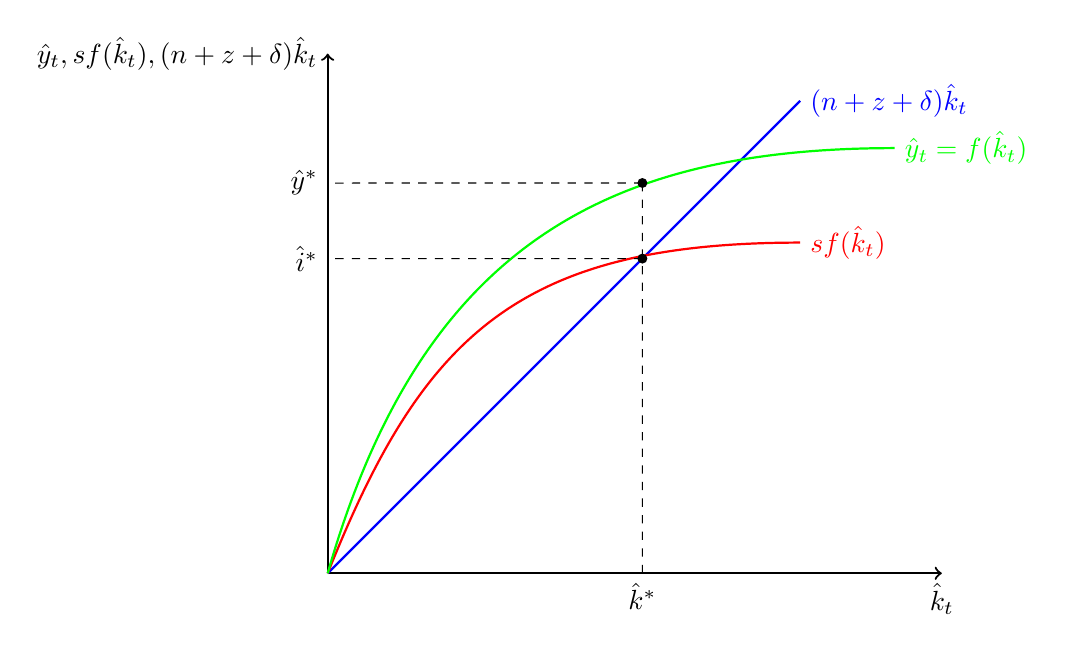
\begin{tikzpicture}[scale=1.2, domain=0:6]
  % Axes
  \draw[thick, ->] (0,0) node[below left] {} -- (6.5,0) node[below] {$\hat{k}_{t}$};
  \draw[thick, ->] (0,0) -- (0,5.5) node[left] {$\hat{y}_{t}, sf(\hat{k}_t), (n+z+\delta)\hat{k}_{t}$};

  % Depreciation line ( \delta k )
  \draw[thick, blue] (0,0) -- (5,5) node[right] {$(n+z+\delta)\hat{k}_{t}$};

  % Saving curve ( sf(k) )
  \draw[thick, red] (0,0) .. controls (1,2.5) and (2,3.5) .. (5,3.5) node[right] {$sf(\hat{k}_{t})$};

  % Saving curve ( sf(k) )
  \draw[thick, green] (0,0) .. controls (1,3.5) and (3,4.5) .. (6,4.5) node[right] {$\hat{y}_{t} = f(\hat{k}_{t})$};

  % Steady state markers
  \coordinate (SS1) at (3.33, 3.33);
  \coordinate (SS2) at (3.33, 4.13);
  \fill[black] (SS1) circle (1.5pt);
  \fill[black] (SS2) circle (1.5pt);
  \draw[dashed] (SS2) -- (3.33,0) node[below] {$\hat{k}^*$};
  \draw[dashed] (SS1) -- (0,3.33) node[left] {$\hat{i}^*$};
  \draw[dashed] (SS2) -- (0,4.13) node[left] {$\hat{y}^*$};
\end{tikzpicture}

\end{document}
    }
\end{figure}

\newpage
\begin{itemize}
\item Using these graphs, we can easily analyze the dynamics when any of the exogenous variable ($s, n, z, \delta$) changes. (Exercise: what if $s$ increases?)
\item Golden rule for saving rate:
\begin{itemize}
\item What is the optimal $s$ that maximizes consumption?
\item Again, we make use of the equation $sf(\hat{k}^*) \approx (n+z+\delta)\hat{k}^*$.
\begin{align*}
\hat{c}^* &= (1-s)f(\hat{k}^*) \\
&= f(\hat{k}^*) - (n+z+\delta)\hat{k}^*
\end{align*}
Taking FOC:
\[
\frac{\partial \hat{c}^*}{\partial s} = (f'(\hat{k}^*) - (n+z+\delta)) \frac{\partial \hat{k}^*}{\partial s} = 0
\]
Since $\frac{\partial \hat{k}^*}{\partial s} > 0$ always, the term $f'(\hat{k}^*) - (n+z+\delta)$ must equal 0.
\[
f'(\hat{k}^*) = n+z+\delta
\]
Example - Cobb-Douglas:
\begin{align*}
\alpha (\hat{k}^*)^{\alpha-1} &= n+z+\delta \\
\alpha \left(\left(\frac{s}{n+z+\delta}\right)^{\frac{1}{1-\alpha}}\right)^{\alpha-1} &= n+z+\delta \\
s^{\text{gr}} &= \alpha
\end{align*}
\item Problem: Because we assume household do not optimize, the model allows $s \ne s^{\text{gr}} \implies$ dynamic inefficiency.
\end{itemize}

\item Does the model explain cross-country convergence?
\begin{itemize}
\item Recall that:
\[
g_{\hat{k}} \approx \frac{s}{(1+n)(1+z)}\cdot\frac{f(\hat{k}_t)}{\hat{k}_t} - \frac{n+z+\delta}{(1+n)(1+z)}
\]
If two countries have the same $s, n, z, \delta$ but $\hat{k}_t^\text{poor} < \hat{k}_t^\text{rich}$, then $g_{\hat{k}}^\text{poor} > g_{\hat{k}}^\text{rich}$, and furthermore they have the same $\hat{k}^*$.
\end{itemize}
\end{itemize}
\begin{figure}[h]
    \centering
    \resizebox{0.6\textwidth}{!}{
    \documentclass{standalone}
\usepackage{tikz}
\usepackage{amsmath}
\begin{document}

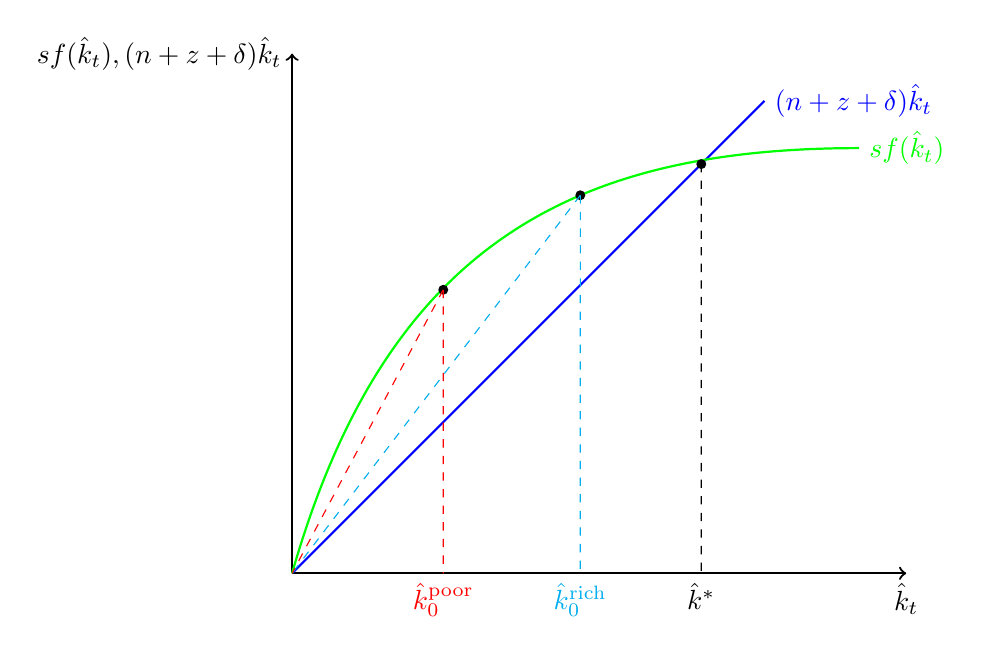
\begin{tikzpicture}[scale=1.2, domain=0:6]
  % Axes
  \draw[thick, ->] (0,0) node[below left] {} -- (6.5,0) node[below] {$\hat{k}_{t}$};
  \draw[thick, ->] (0,0) -- (0,5.5) node[left] {$sf(\hat{k}_{t}), (n+z+\delta)\hat{k}_{t}$};

  % Depreciation line ( \delta k )
  \draw[thick, blue] (0,0) -- (5,5) node[right] {$(n+z+\delta)\hat{k}_{t}$};

  % Saving curve ( sf(k) )
  \draw[thick, green] (0,0) .. controls (1,3.5) and (3,4.5) .. (6,4.5) node[right] {$sf(\hat{k}_{t})$};

  % Steady state markers
  \coordinate (SS) at (4.33, 4.33);
  \coordinate (rich) at (3.05, 4);
  \coordinate (poor) at (1.6, 3);
  \fill[black] (SS) circle (1.5pt);
  \fill[black] (rich) circle (1.5pt);
  \fill[black] (poor) circle (1.5pt);
  \draw[dashed] (SS) -- (4.33,0) node[below] {$\hat{k}^*$};
  \draw[cyan, dashed] (rich) -- (3.05,0) node[below] {$\hat{k}^\text{rich}_0$};
  \draw[cyan, dashed] (rich) -- (0,0);
  \draw[red, dashed] (poor) -- (1.6,0) node[below] {$\hat{k}^\text{poor}_0$};
  \draw[red, dashed] (poor) -- (0,0);
\end{tikzpicture}

\end{document}
    }
\end{figure}
\begin{itemize}
\item[]
\begin{itemize}
\item The slope of the hypotenuse $= \frac{sf(\hat{k}_t)}{\hat{k}_t}$ tells us about $g_{\hat{k}}$, and clearly the poor economy has a steeper slope and thus a higher growth rate.
\item This aligns with conditional convergence.
\item What if the two countries have different $s$?
\end{itemize}
\end{itemize}
\begin{figure}[h]
    \centering
    \resizebox{0.6\textwidth}{!}{
    \documentclass{standalone}
\usepackage{tikz}
\usepackage{amsmath}
\begin{document}

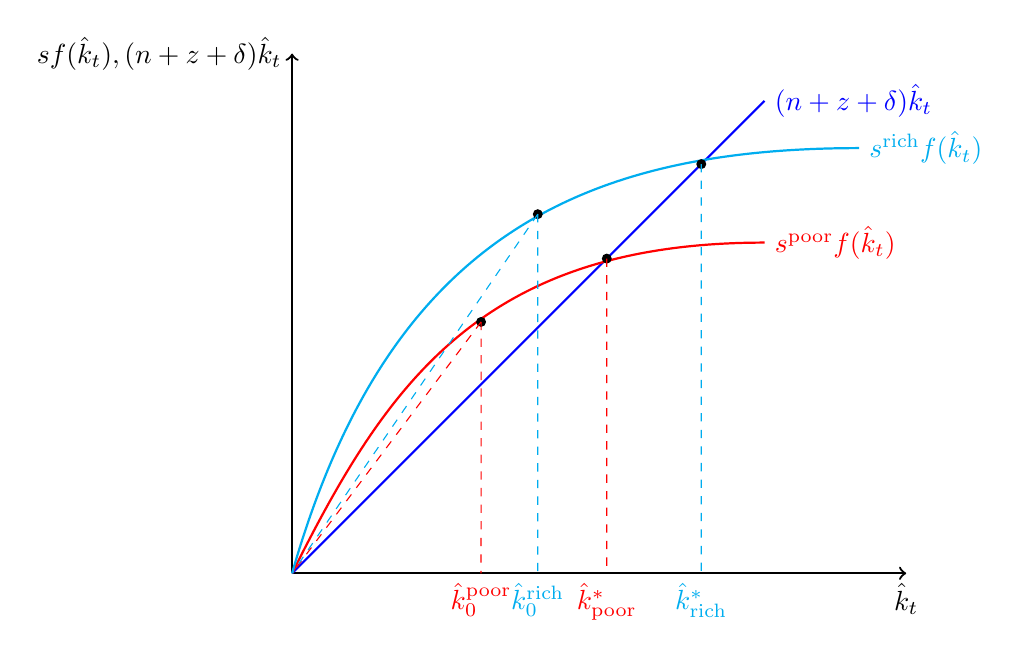
\begin{tikzpicture}[scale=1.2, domain=0:6]
  % Axes
  \draw[thick, ->] (0,0) node[below left] {} -- (6.5,0) node[below] {$\hat{k}_{t}$};
  \draw[thick, ->] (0,0) -- (0,5.5) node[left] {$sf(\hat{k}_{t}), (n+z+\delta)\hat{k}_{t}$};

  % Depreciation line ( \delta k )
  \draw[thick, blue] (0,0) -- (5,5) node[right] {$(n+z+\delta)\hat{k}_{t}$};

  % Saving curve ( sf(k) )
  \draw[thick, red] (0,0) .. controls (1,2) and (2,3.5) .. (5,3.5) node[right] {$s^\text{poor}f(\hat{k}_{t})$};

  % Saving curve ( sf(k) )
  \draw[thick, cyan] (0,0) .. controls (1,3.5) and (3,4.5) .. (6,4.5) node[right] {$s^\text{rich}f(\hat{k}_{t})$};

  % Steady state markers
  \coordinate (poorss) at (3.33, 3.33);
  \fill[black] (poorss) circle (1.5pt);
  \coordinate (richss) at (4.33, 4.33);
  \fill[black] (richss) circle (1.5pt);
  \coordinate (rich) at (2.6, 3.8);
  \fill[black] (rich) circle (1.5pt);
  \coordinate (poor) at (2, 2.66);
  \fill[black] (poor) circle (1.5pt);
  \draw[red, dashed] (poorss) -- (3.33,0) node[below] {$\hat{k}^*_\text{poor}$};
  \draw[cyan, dashed] (richss) -- (4.33,0) node[below] {$\hat{k}^*_\text{rich}$};
  \draw[red, dashed] (poor) -- (2,0) node[below] {$\hat{k}^\text{poor}_0$};
  \draw[cyan, dashed] (rich) -- (2.6,0) node[below] {$\hat{k}^\text{rich}_0$};
  \draw[red, dashed] (poor) -- (0,0);
  \draw[cyan, dashed] (rich) -- (0,0);
\end{tikzpicture}

\end{document}
    }
\end{figure}
\begin{itemize}
\item[]
\begin{itemize}
\item In this case, the rich country has higher growth rate.
\item Rejects absolute convergence.
\item Although the model explains the facts about convergence qualitatively, empirical data shows that the the predicted convergence rate is too fast.
\end{itemize}

\item Does the model explain cross-country different in output per capita?
\begin{itemize}
\item Difference in $\frac{K}{N}$?
\begin{itemize}
\item Consider $\tilde{y}_1 = \frac{Y_1}{N_1} = \left(\frac{K_1}{N_1}\right)^\alpha Z^{1-\alpha}$ and $\tilde{y}_2 = \frac{Y_2}{N_2} = \left(\frac{K_2}{N_2}\right)^\alpha Z^{1-\alpha}$.
\item If $\frac{\tilde{y}_1}{\tilde{y}_2} = X$, then their $\frac{K}{N}$ must differ by $X^\frac{1}{\alpha}$. If $X=10$ and $\alpha=\frac{1}{3}$, the difference in $\frac{K}{N}$ must be 1000 times.
\item Not plausible.
\end{itemize}
\item Difference in $s$?
\begin{itemize}
\item Textbook exercise.
\end{itemize}
\item Difference in $Z$?
\item How to measure technology / productivity exactly?
\begin{align*}
Y_t &= A_tK^\alpha_t(Z_tN_t)^{1-\alpha} \\
\ln Y_t &= \ln A_t + \alpha \ln K_t + (1-\alpha) \ln Z_t + (1-\alpha) \ln N_t
\end{align*}
Define total factor productivity (TFP) as the proportion of income growth that cannot be attributed to $K_t$ or $N_t$.
\[
\ln \text{TFP}_t = \ln A_t + (1-\alpha) \ln Z_t = \ln Y_t - \alpha \ln K_t - (1-\alpha) \ln N_t
\]
\item Young (1992): Growth in HK can be explained by growth in technology, but not in Singapore.
\item Still, correlation between GDP and TDP is high in broader sample.
\item Solow model predicts sustained growth must be driven by productivity $Z_t$, but does not explain what productivity is.
\item Some factors affecting productivity: Knowledge and education, Climate, Geography, Institution, Finance, Degree of openness
\item Policy implication: Focus on policies that promote productivity.
\end{itemize}
\end{itemize}

\section{Consumption}
\begin{itemize}
\item Previously we assumed consumer do not choose savings to optimize their consumption.
\item We can use a simple two-period model to analyze consumption behavior.
\item Assumptions:
\begin{itemize}
\item Two periods: $t$ and $t+1$.
\item Exchange economy. No money, no production, only endowment.
\item A representative consumer.
\end{itemize}
\item Budget constraints: 
\begin{itemize}
\item Period $t$:
\begin{equation*}
C_t + S_t = Y_t \label{(1)}
\end{equation*}
\item Period $t+1$:
\begin{equation*}
C_{t+1} + S_{t+1} = Y_{t+1} + (1+r)S_t
\end{equation*}
Household would not allow $S_{t+1} > 0$ as there is no next period to consume. Lenders would not lend for $S_{t+1} < 0$ as the household would not repay. Thus the terminal condition is $S_{t+1} = 0$.
\begin{equation*}
C_{t+1} = Y_{t+1} + (1+r_t)S_t
\end{equation*}
\item Combining the two equations by letting $S_t$ equal each other, we have the intertemporal budget constraint:
\[
C_t + \frac{C_{t+1}}{1+r_t} = Y_t + \frac{Y_{t+1}}{1+r_t}
\]
\item PDV of consumption = PDV of income.
\end{itemize}

\item Utility:
\begin{itemize}
\item $u'(C) > 0, u''(C) < 0.$
\item Total utility: $U(C_t, C_{t+1}) = u(C_t) + \beta u(C_{t+1})$, where $0 < \beta < 1$.
\end{itemize}

\item The maximization problem:
\[
\max_{C_t, C_{t+1}} U(C_t, C_{t+1}) = u(C_t) + \beta u(C_{t+1})
\]
\[
\text{s.t. } C_t + \frac{C_{t+1}}{1+r_t} = Y_t + \frac{Y_{t+1}}{1+r_t}
\]
Setting up the Lagrangian:
\[
\mathcal{L}(C_t, C_{t+1}, \lambda) = u(C_t) + \beta u(C_{t+1}) + \lambda (Y_t + \frac{Y_{t+1}}{1+r_t} - C_t + \frac{C_{t+1}}{1+r_t})
\]
Taking FOCs:
\begin{align*}
\begin{cases}
\frac{\partial \mathcal{L}}{\partial C_{t}} = u'(C_t) - \lambda = 0 \\
\frac{\partial \mathcal{L}}{\partial C_{t+1}} = \beta u'(C_{t+1}) - \frac{\lambda}{1+r_t} = 0
\end{cases}
\end{align*}
Setting $\lambda$ equal each other, we can get the Euler equation:
\[
u'(C_t) = \beta(1+r_t)u'(C_{t+1})
\]
The intuition: MB = MC of present consumption.
\item Substituting the budget constraint $C_{t+1} = (1+r_t)Y_t + Y_{t+1} - (1+r_t)C_t$ into the Euler equation, we can find the consumption function:
\[
C_t = C^d(Y_t, Y_{t+1}, r_t)
\]

\item Example - log utility: $u(C) = \ln C$.
\begin{itemize}
\item The Euler equation:
\[
\frac{1}{C_t} = \beta(1+r_t)\frac{1}{C_{t+1}} \implies C_{t+1} = \beta(1+r_t)C_t
\]
Hence,
\begin{align*}
\beta(1+r_t)C_t &= (1+r_t)Y_t + Y_{t+1} - (1+r_t)C_t \\
C_t &= \left(\frac{1}{1+\beta}\right)\left(Y_t + \frac{Y_{t+1}}{1+r_t}\right)
\end{align*}
\end{itemize}

\item The indifference curve:
\begin{itemize}
\item Recall that $U = u(C_t) + \beta u(C_{t+1})$.
\item To find the slope of the indifference curve, a shortcut is using the implicit function theorem:
\[
\frac{d C_{t+1}}{dC_t} = -\frac{\frac{\partial U}{\partial C_t}}{\frac{\partial U}{\partial C_{t+1}}} = - \frac{u'(C_t)}{\beta u'(C_{t+1})}
\]
At the optimum consumption point, by the Euler equation, $u'(C_t) = \beta(1+r_t)u'(C_{t+1})$. Thus, at the point, the slope to the indifference curve is:
\[
\frac{d C_{t+1}}{dC_t} = -(1+r_t)
\]
Which we can see that the budget line exactly tangents to the point:
\[
C_{t+1} = (1+r_t)Y_t + Y_{t+1} - (1+r_t)C_t
\]
\end{itemize}
\end{itemize}

\begin{figure}[h]
    \centering
    \resizebox{0.7\textwidth}{!}{
    \documentclass{standalone}
\usepackage{tikz}

\begin{document}
\begin{tikzpicture}[scale=1.5]
    % Draw axes
    \draw[->, thick] (0,0) -- (6,0) node[right] {$C_t$};
    \draw[->, thick] (0,0) -- (0,5) node[above] {$C_{t+1}$};

    % Draw budget constraint line
    % Y-intercept: C_t = 0 => C_{t+1} = (1+r_t)Y_t + Y_{t+1}
    % X-intercept: C_{t+1} = 0 => C_t = Y_t + Y_{t+1}/(1+r_t)
    \draw[thick, blue] (0,4) node[left] {$(1+r_t)Y_t + Y_{t+1}$} -- (5,0) node[below] {$Y_t + \frac{Y_{t+1}}{1+r_t}$};

    % Draw indifference curve tangent to the budget line
    % Draw strictly convex indifference curve tangent to the budget line at (2.5, 2)
    % Using explicit Bezier controls aligned with the tangent slope (-0.8)
    \draw[thick, red] (0.5, 4.5) 
        .. controls (0.8, 3.5) and (1.5, 2.8) .. (2.5, 2) 
        .. controls (3.5, 1.2) and (4.5, 0.7) .. (5.5, 0.5) node[right] {};


    % Mark the optimal consumption point (tangency)
    \filldraw[black] (2.5,2) circle (1.5pt);
    \draw[dashed] (2.5,0) node[below] {$C_t^*$} -- (2.5,2) -- (0,2) node[left] {$C_{t+1}^*$};
    
\end{tikzpicture}
\end{document}

    }
\end{figure}

\begin{itemize}
\item The graphical analysis of dynamics is omitted, but here we discuss the result verbally.

\item Increase in $Y_t$ or $Y_{t+1}$:
\begin{itemize}
\item Given an \textbf{income effect}, since both $C_t$ and $C_{t+1}$ are normal goods, both $C^*_t$ and $C^*_{t+1}$ should increase.
\item \textbf{Consumption smoothing}: If the income in \textbf{either} period increases, the consumer will consume the increase across \textbf{both} periods.
\item 0 $<$ MPC $<$ 1.
\end{itemize}

\item Increase in $r_t$:
\begin{itemize}
\item An important note: the consumption bundle $(Y_t, Y_{t+1})$ lies on the budget line.
\item Then, we can classify the consumer into two types.
\item Saver: $C^*_t < Y_t$
\begin{itemize}
\item Substitution effect: $C_t \downarrow, C_{t+1} \uparrow$
\item Income effect: $C_t \uparrow, C_{t+1} \uparrow$
\item Overall: $C_t ?, C_{t+1} \uparrow$
\end{itemize}
\item Borrower: $C^*_t > Y_t$
\begin{itemize}
\item Substitution effect: $C_t \downarrow, C_{t+1} \uparrow$
\item Income effect: $C_t \downarrow, C_{t+1} \downarrow$
\item Overall: $C_t \downarrow, C_{t+1}?$
\end{itemize}
\end{itemize}

\item Oftentimes we will assume substitution effect dominates $\implies \frac{\partial C_t}{\partial r_t} < 0$.

\item Revisiting the log utility example, where $C_t = \left(\frac{1}{1+\beta}\right)\left(Y_t + \frac{Y_{t+1}}{1+r_t}\right)$.
\[
\frac{\partial C_t}{\partial Y_t} = \frac{1}{1+\beta} < 1
\]
\[
\frac{\partial C_t}{\partial Y_{t+1}} = \frac{1}{(1+\beta)(1+r_t)} < 1
\]
\[
\frac{\partial C_t}{\partial r_t} = -\left(\frac{1}{1+\beta}\right)\left(\frac{Y_{t+1}}{(1+r_t)^2}\right) < 0
\]

\item Permanent income hypothesis: Consumption is a function of the present discounted value of the lifetime income.
\begin{itemize}
\item Holds for the log utility case.
\end{itemize}

\item When $Y_t$ increases,
\[
dC_t = \frac{\partial C^d(\cdot)}{\partial Y_t}dY_t + \frac{\partial C^d(\cdot)}{\partial Y_{t+1}} dY_{t+1}+ \frac{\partial C^d(\cdot)}{\partial r_t}dr_t
\]
\begin{itemize}
\item If the increase is a transitory income ($dY_t>0,dY_{t+1}=0$):
\[
\frac{dC_t}{dY_t} = \frac{\partial C^d(\cdot)}{\partial Y_t}
\]
\item If the increase is a permanent income ($dY_t=dY_{t+1}>0$):
\[
\frac{dC_t}{dY_t} = \frac{\partial C^d(\cdot)}{\partial Y_t} + \frac{\partial C^d(\cdot)}{\partial Y_{t+1}}
\]
\end{itemize}

\item What if $Y_{t+1}$ is uncertain?
\begin{itemize}
\item Let $Y_{t+1}$ be a random variable.
\begin{align*}
Y_{t+1} &=
\begin{cases}
Y^H_{t+1} = Y_t + \Delta \text{ with probability } p \\
Y^L_{t+1} = Y_t - \Delta \text{ with probability } 1-p
\end{cases}
\end{align*}
\iffalse
\item Then, $C_{t+1}$ is also a random variable.
\begin{align*}
C_{t+1} &=
\begin{cases}
C^H_{t+1} = Y^H_{t+1} + (1+r_t)S_t \text{ with probability } p \\
C^L_{t+1} = Y^L_{t+1} + (1+r_t)S_t \text{ with probability } 1-p
\end{cases}
\end{align*}
\fi
\item The expression for the intertemporal budget constraint remains the same, except that $Y_{t+1}$ and $C_{t+1}$ are now random variables.
\item Recall the fact that $\mathbb{E}(u(X))=\sum p_i u(x_i)$, and thus $\mathbb{E}(u'(X))=\sum p_i u'(x_i)$.
\item Solve for the maximization problem:
\[
\max_{C_t, C_{t+1}} U(C_t, C_{t+1}) = u(C_t) + \beta \mathbb{E}(u(C_{t+1}))
\]
\[
\text{s.t. } C_t + \frac{C_{t+1}}{1+r_t} = Y_t + \frac{Y_{t+1}}{1+r_t}
\]
Setting up the Lagrangian:
\[
\mathcal{L}(C_t, C_{t+1}, \lambda) = u(C_t) + \beta \mathbb{E}(u(C_{t+1})) + \lambda (Y_t + \frac{Y_{t+1}}{1+r_t} - C_t + \frac{C_{t+1}}{1+r_t})
\]
Taking FOCs:
\begin{align*}
\begin{cases}
\frac{\partial \mathcal{L}}{\partial C_{t}} = u'(C_t) - \lambda = 0 \\
\frac{\partial \mathcal{L}}{\partial C_{t+1}} = \beta \mathbb{E}(u'(C_{t+1})) - \frac{\lambda}{1+r_t} = 0
\end{cases}
\end{align*}
Setting $\lambda$ equal each other, we can get the Euler equation:
\[
u'(C_t) = \beta(1+r_t)\mathbb{E}(u'(C_{t+1}))
\]
\item Since $\mathbb{E}(u'(C_{t+1})) \ne u'(\mathbb{E}(C_{t+1}))$ most of the time (Jensen's inequality), this is difficult to solve.
\item For example, for log utility, $\mathbb{E}\left(\frac{1}{C_{t+1}}\right) \ne \frac{1}{\mathbb{E}(C_{t+1})}$.
\item Special case: Quadratic utility.
\item Will people save more if future income is more uncertain? (Precautionary saving)
\item Yes, if $u'(C)$ is convex $\iff u'''(C) > 0$.
\end{itemize}
\end{itemize}
\begin{figure}[h]%
    \centering
    \resizebox{0.48\textwidth}{!}{\documentclass{standalone}
\usepackage{tikz}
\usepackage{amssymb}

\begin{document}
\begin{tikzpicture}[scale=1.5]
    % Draw axes
    \draw[->, thick] (0,0) -- (5.5,0) node[right] {$C_{t+1}$};
    \draw[->, thick] (0,0) -- (0,5) node[above] {$U'(C_{t+1})$};


    % Draw indifference curve tangent to the budget line
    % Draw strictly convex indifference curve tangent to the budget line at (2.5, 2)
    % Using explicit Bezier controls aligned with the tangent slope (-0.8)
    \draw[blue] (0.5, 4.5) .. controls (0.8, 0.8) and (2.5, 0.6) .. (5, 0.5);

    % Markers
    \coordinate (L) at (1.25, 1.85);
    \fill[black] (L) circle (1.5pt);
    \draw[cyan, dashed] (L) -- (1.25, 0) node[below] {$C_{t+1}^L$};
    \draw[cyan, dashed] (L) -- (0, 1.85) node[left] {$u'(C_{t+1}^L)$};

    \coordinate (H) at (2.5, 0.85);
    \fill[black] (H) circle (1.5pt);
    \draw[red, dashed] (H) -- (2.5, 0) node[below] {$C_{t+1}^H$};
    \draw[red, dashed] (H) -- (0, 0.85) node[left] {$u'(C_{t+1}^H)$};

    \coordinate (M) at (1.875, 1.35);
    \fill[black] (M) circle (1.5pt);
    \draw[black, dashed] (M) -- (1.875, 0) node[below] {$\mathbb{E}(C_{t+1})$};
    \draw[black, dashed] (M) -- (0, 1.35) node[left] {$\mathbb{E}(u'(C_{t+1}))$};
    
    \draw[red, dashed] (L) -- (H);
    
\end{tikzpicture}
\end{document}
}%
    \hfill
    \resizebox{0.48\textwidth}{!}{\input{precautionary2}}%
\end{figure}
\begin{itemize}
\item[]
\begin{itemize}
\item The higher the variance, the higher $\mathbb{E}(u'(C_{t+1}))$. By the Euler equation, $u'(C_t)$ is higher, and because $u'(C_t)$ is strictly decreasing with $C_t$, $C_t$ becomes lower and people save more instead.
\item Intuition: MC of consumption $= u'(C_t)$ is high.
\item For example, consumption was low after the Great Recession due to high future uncertainty.
\item Mathematical property: mean-preserving spread ($u'(C_{t+1}^L)$ increases much faster than $u'(C_{t+1}^H)$ decreases).
\end{itemize}

\item Therefore, consumers have two motives to save or borrow: consumption smoothing ($u''(C)<0$) and risk aversion ($u'''(C)>0$).

\item Random walk hypothesis:
\begin{itemize}
\item Without expectation, if $\beta = \frac{1}{1+r}$, then $u'(C_t) = u'(C_{t+1}) \implies C_t = C_{t+1}$.
\item With expectation, $u'(C_t) = \mathbb{E}(u'(C_{t+1})) \implies C_t = \mathbb{E}(C_{t+1})$ only if $u'''(C) = 0$.
\end{itemize}
\end{itemize}

\section{General Equilibrium}
\begin{itemize}
\item While we just assumed $r_t$ to be exogenous, in an economy with many agents, $r_t$ is actually determined endogenously by clearing the borrowing and lending market.
\item First, we assume there are many households with the same preference. Each of the households, indexed by $j$, maximize their own utility by the standard formulation:
\[
\max_{C_{j,t}, C_{j,t+1}} u(C_{j,t}) + \beta u(C_{j,t+1})
\]
\[
\text{s.t. } C_{j,t} + \frac{C_{j,t+1}}{1+r_t} = Y_{j,t} + \frac{Y_{j,t+1}}{1+r_t}
\]
Then, we can obtain:
\[
C_{j,t} = C^d(Y_{j,t}, Y_{j,t+1}, r_t)
\]
\item All markets clear, since every borrower must be matched with a reciprocal lender, the condition for aggregate savings $S_t$ must be:
\[
S_t = \sum S_{j,t} = 0
\]
\item Then,
\[
\sum Y_{j,t} = \sum C_{j,t}
\]
Which gives us a nice relationship between aggregate income $Y_t$ and consumption $C_t$:
\[
Y_t = C_t = C^d_t(Y_t, Y_{t+1}, r_t)
\]
We can then use this to find the equilibrium $r_t$.
\item Example - log utility:
\begin{align*}
Y_t &= \frac{1}{1+\beta}\left(Y_t + \frac{Y_{t+1}}{1+r_t}\right) \\
r_t &= \frac{1}{\beta} \cdot \frac{Y_{t+1}}{Y_t}
\end{align*}

\item Note that we only assume everyone has the same preference. If households have different endowments, the conditions will still hold.

\item This is the market demand, what about the supply?
\item In an endowment economy, there is no production and $Y_t$ is exogenously given. The supply is just a vertical line.

\item Graphical representation:
\begin{itemize}
\item Assume substitution effect dominates, so $C^d_t(Y_t, Y_{t+1}, r_t)$ is decreasing in $r_t$.
\item The slope $= \frac{\partial C^d_t}{\partial Y_t} = \text{MPC}$, $0 < \text{MPC} < 1$.
\end{itemize}

\begin{figure}[h]
    \centering
    \resizebox{0.5\textwidth}{!}{
    \documentclass[border=10pt]{standalone}
\usepackage{tikz}
\usepackage{xcolor}
\usepackage{amsmath}

\begin{document}
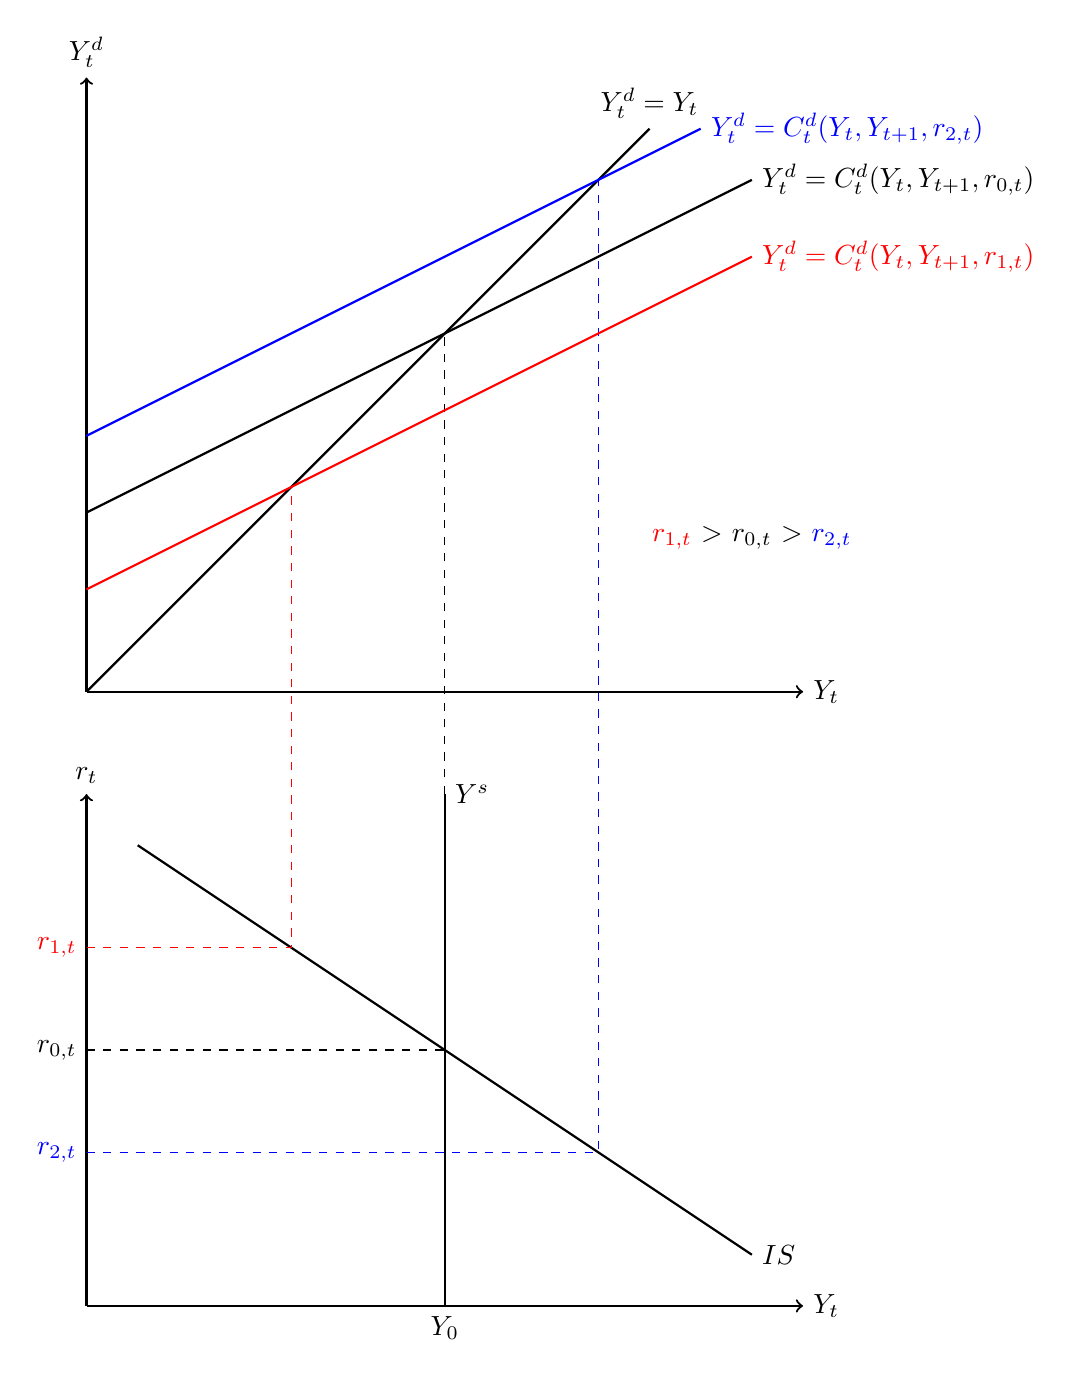
\begin{tikzpicture}[scale=1.3]

    % ==========================================
    % BOTTOM GRAPH: IS Curve Derivation
    % ==========================================
    
    % Axes
    \draw[thick, ->] (0,0) -- (7,0) node[right] {$Y_t$};
    \draw[thick, ->] (0,0) -- (0,5) node[above] {$r_t$};

    % IS Curve
    \draw[thick] (0.5, 4.5) -- (6.5, 0.5) node[right] {$IS$};

    % Y^s Vertical Line
    \draw[thick] (3.5, 0) node[below] {$Y_0$} -- (3.5, 5) node[right] {$Y^s$};

    % Dashed lines and interest rate labels
    % High interest rate (r1) -> low output
    \draw[dashed, red] (0, 3.5) node[left] {$r_{1,t}$} -- (2, 3.5) -- (2, 8);
    
    % Equilibrium interest rate (r0) -> medium output
    \draw[dashed, black] (0, 2.5) node[left] {$r_{0,t}$} -- (3.5, 2.5) -- (3.5, 9.5);
    
    % Low interest rate (r2) -> high output
    \draw[dashed, blue] (0, 1.5) node[left] {$r_{2,t}$} -- (5, 1.5) -- (5, 11);


    % ==========================================
    % TOP GRAPH: Keynesian Cross
    % ==========================================
    
    % Shift coordinate system up by 6cm for the top graph
    \begin{scope}[yshift=6cm]
        % Axes
        \draw[thick, ->] (0,0) -- (7,0) node[right] {$Y_t$};
        \draw[thick, ->] (0,0) -- (0,6) node[above] {$Y_t^d$};

        % 45-degree line (Y = Y^d)
        \draw[thick] (0,0) -- (5.5, 5.5) node[above] {$Y_t^d = Y_t$};

        % Aggregate Demand Curves
        % Bottom AD curve (Red - highest interest rate)
        \draw[thick, red] (0, 1) -- (6.5, 4.25) node[right] {$Y_t^d = C_t^d(Y_t, Y_{t+1}, r_{1,t})$};
        
        % Middle AD curve (Black - middle interest rate)
        \draw[thick, black] (0, 1.75) -- (6.5, 5.0) node[right] {$Y_t^d = C_t^d(Y_t, Y_{t+1}, r_{0,t})$};
        
        % Top AD curve (Blue - lowest interest rate)
        \draw[thick, blue] (0, 2.5) -- (6.0, 5.5) node[right] {$Y_t^d = C_t^d(Y_t, Y_{t+1}, r_{2,t})$};

        % Inequality text indicating the relationship between interest rates
        \node at (6.5, 1.5) {\textcolor{red}{$r_{1,t}$} $>$ $r_{0,t}$ $>$ \textcolor{blue}{$r_{2,t}$}};
    \end{scope}

\end{tikzpicture}
\end{document}
    }
\end{figure}

\end{itemize}

\section{Production Economy}

\begin{itemize}
\item Now, we can introduction firms to move from an endowment economy to a production economy.
\item Firm:
\begin{itemize}
\item We still use a CRTS and diminishing (e.g. Cobb-Douglas) production function, but not labor augmenting (i.e. no $Z_t$) for simplicity.
\[
Y_t = A_t F(K_t, N_t)
\]
\item Capital accumulation equation:
\[
K_{t+1} = I_t + (1-\delta)K_t 
\]
In other words, if the firm simply chooses $K_{t+1}$, investment is implicitly defined by:
\[
I_t = K_{t+1} - (1-\delta)K_t 
\]
\item The firm finances investment through borrowing with a premium $f_t$, so the cost of borrowing is:
\[
r_t' = r_t + f_t
\]
\item Dividends:
\begin{itemize}
\item Period $t$: The dividend is simply the profit: income minus labor cost.
\[
D_t = Y_t - w_tN_t
\]
\item Period $t+1$: In addition to profits, since the firm ceases to exist, it liquidates the remaining capital. Also, it needs to repay the cost of debt.
\[
D_{t+1} = Y_{t+1} + (1-\delta)K_{t+1} - w_{t+1}N_{t+1} - (1+r'_t)I_t
\]
\end{itemize}
\item The firm maximizes the firm value, which is the PDV of dividends, by choosing $N_t$ and $K_{t+1}$. Note that all other variables, including $K_t$, are exogenously given. Substituting everything:
\begin{align*}
\max_{N_t, K_{t+1}} V_t 
&= D_t + \left(\frac{1}{1+r_t}\right)D_{t+1} \\
&= A_t F(K_t, N_t) - w_tN_t +\left(\frac{1}{1+r_t}\right) (A_{t+1} F(K_{t+1}, N_{t+1}) + (1-\delta)K_{t+1} \\
&- w_{t+1}N_{t+1} - (1+r'_t)(K_{t+1} - (1-\delta)K_t ))
\end{align*}
\item Taking FOCs gives us the labor and investment demands respectively.
\item Labor demand:
\begin{align*}
\frac{\partial V_t}{\partial N_t} = A_tF_N(K_t, N_t) - w_t &= 0 \\
w_t &= A_tF_N(K_t, N_t)
\end{align*}
\begin{itemize}
\item The effects on $N_t$ if each of the variables moves:
\item $w_t \uparrow \implies F_N(K_t, N_t) \uparrow \implies N_t \downarrow$
\item $A_t \uparrow \implies F_N(K_t, N_t) \downarrow \implies N_t \uparrow$
\item $K_t \uparrow, F_N(K_t, N_t) \sim \implies N_t \downarrow$
\item Therefore, the labor demand function (with symbols for relations) is:
\[
N_t = N^d_t(w_t^-, A_t^+, K_t^-)
\]
\end{itemize}

\item Investment demand:
\begin{align*}
\frac{\partial V_t}{\partial K_{t+1}} = \left(\frac{1}{1+r_t}\right) (A_{t+1}F_K(K_{t+1}, N_{t+1}) + (1-\delta) - (1+r_t')) &= 0 \\
1+r'_t &= A_{t+1}F_K(K_{t+1}, N_{t+1}) + (1-\delta)
\end{align*}
\begin{itemize}
\item Intuition: MB = MC of investment.
\item Further rearranging:
\[
r_t+f_t+\delta = A_{t+1}F_K(K_{t+1}, N_{t+1})
\]
\item Recall:
\[
I_t = K_{t+1} - (1-\delta)K_t 
\]
\item The effects on $I_t$ if each of the variables moves:
\item $r_t \uparrow \implies F_K(K_{t+1}, N_{t+1}) \uparrow \implies K_{t+1} \downarrow \implies I_t \downarrow$
\item $f_t \uparrow \implies F_K(K_{t+1}, N_{t+1}) \uparrow \implies K_{t+1} \downarrow \implies I_t \downarrow$
\item $A_{t+1} \uparrow \implies F_N(K_t, N_t) \downarrow \implies K_{t+1} \uparrow \implies I_t \uparrow$
\item $K_t \uparrow \implies I_t \downarrow$
\item Therefore, the investment demand function is:
\[
I_t = I^d_t(r_t^-, A_{t+1}^+, f_t^-, K_t^-)
\]
\end{itemize}
\end{itemize}
\end{itemize}

\begin{figure}[h]
    \centering
    \resizebox{0.2\textwidth}{!}{\documentclass{standalone}
\usepackage{tikz}

\begin{document}
\begin{tikzpicture}[scale=1.2]

    % Draw Axes
    \draw[thick, <->] (0, 5) node[left] {$w_t$} -- (0, 0) -- (5, 0) node[below] {$N_t$};
    
    % Draw Demand Curve
    \draw[thick, blue] (0.5, 4) -- (4, 0.5) node[right] {$N^d(w_t,A_t,K_t)$};

\end{tikzpicture}
\end{document}}%
    \quad
    \resizebox{0.2\textwidth}{!}{\documentclass{standalone}
\usepackage{tikz}

\begin{document}
\begin{tikzpicture}[scale=1.2]

    % Draw Axes
    \draw[thick, <->] (0, 5) node[left] {$r_t$} -- (0, 0) -- (5, 0) node[below] {$I_t$};
    
    % Draw Demand Curve
    \draw[thick, blue] (0.5, 4) -- (4, 0.5) node[right] {$I^d_t(r_t, A_{t+1}, f_t, K_t)$};

\end{tikzpicture}
\end{document}}%
\end{figure}

\begin{itemize}
\item Household:
\begin{itemize}
\item In addition to consumption, household also enjoy leisure, which is simply defined by:
\[
L_t = 1 - N_t
\]
\item Thus, the total utility is:
\[
U = u(C_t, 1-N_t) + \beta u(C_{t+1}, 1-N_{t+1})
\]
\item Period $t$: Household earns labor income and dividends:
\[
C_t + S_t = w_tN_t + D_t
\]
\item Period $t+1$: Household also gains interest from savings and lending.
\[
C_{t+1} = w_{t+1}N_{t+1} + D_{t+1} + D'_{t+1} + (1+r_t)S_t
\]
\item Combining, we get the intertemporal budget constraint:
\[
C_t + \frac{C_{t+1}}{1+r_t} = w_tN_t + D_t + \frac{w_{t+1}N_{t+1} + D_{t+1} + D'_{t+1} 
}{1+r_t}
\]
\item We can directly put the expression of $C_{t+1}$ into the utility function to get an unconstrained maximization problem: 
\[
\max_{C_t, N_t, N_{t+1}} u(C_t, N_t) + \beta u((1+r_t)(w_tN_t + D_t) + w_{t+1}N_{t+1} + D_{t+1} + D'_{t+1}- (1+r_t)C_t, 1-N_{t+1})
\]
\item Taking FOCs:
\begin{align*}
\begin{cases}
\frac{\partial U}{\partial C_t} = u_C(C_t, 1-N_t) - (1+r_t) \beta u_C(C_{t+1}, 1-N_{t+1}) = 0 \\
\frac{\partial U}{\partial N_t} = -(C_t, 1-N_t) +(1+r_t) \beta w_t u_C(C_{t+1}, 1-N_{t+1}) = 0 \\
\frac{\partial U}{\partial N_{t+1}} = w_t\beta u_C(C_{t+1}, 1-N_{t+1}) - \beta u_L(C_{t+1}, 1-N_{t+1}) = 0
\end{cases}
\end{align*}
Rearranging, we have:
\begin{align*}
\begin{cases}
u_C(C_t, 1-N_t) = (1+r_t) \beta u_C(C_{t+1}, 1-N_{t+1})  \\
u_L(C_t, 1-N_t) = (1+r_t) \beta w_t u_C(C_{t+1}, 1-N_{t+1}) = w_t u_C(C_t, 1-N_t)\\
u_L(C_{t+1}, 1-N_{t+1}) = w_t u_C(C_{t+1}, 1-N_{t+1}) 
\end{cases}
\end{align*}
\item The first equation is the Euler equation, which we have used to simplify the second one.
\item Intuitions: MB = MC of consumption / leisure.
\item Consumption demand is the same as before:
\[
C_t = C^d(Y_t^+, Y_{t+1}^+, r_t^-)
\]
or if we have a government, by Ricardian equivalence:
\[
C_t = C^d((Y_t-G_t)^+, (Y_{t+1}-G_{t+1})^+, r_t^-)
\]
\item The labor supply is more complicated to derive, so we use some assumptions.
\item Specifically, we assume there is no income effect (wages increase, consume more, work less), but only substitution effect (work more because wages increase).
\item Then, the labor supply function is:
\[
N_t = N^s(w_t^+, \theta_t^-)
\]
where $\theta_t$ represents how much one enjoys leisure.

\end{itemize}
\end{itemize}

\begin{figure}[h]
    \centering
    \resizebox{0.3\textwidth}{!}{
    \documentclass{standalone}
\usepackage{tikz}

\begin{document}
\begin{tikzpicture}[scale=1.2]

    % Draw Axes
    \draw[thick, <->] (0, 5) node[left] {$w_t$} -- (0, 0) -- (5, 0) node[below] {$N_t$};
    
    % Draw Demand Curve
    \draw[thick, blue] (0.5, 0.5) -- (4, 4) node[right] {$N^s(w_t,\theta_t)$};

\end{tikzpicture}
\end{document}
    }
\end{figure}

\begin{itemize}
\item []
\begin{itemize}
\item Example - GHH preferences: $u(C, 1-N) = \ln(C+\theta\ln(1-N))$
\end{itemize}
\end{itemize}

\begin{itemize}
\item Market-clearing conditions: Investment = Savings.
\[
I_t = S_t
\]
Then,
\begin{align*}
D_{t+1}' &= (r_t+f_t)I_t-r_tS_t  \\
&= f_tI_t
\end{align*}
Also,
\[
Y_t = w_tN_t + D_t = C_t + S_t = C_t + I_t
\]
or adding government spending:
\[
Y_t = C_t + I_t + G_t
\]
\end{itemize}

\section{Neoclassical RBC Model}

\begin{itemize}
\item To sum up everything we have:
\begin{itemize}
\item Household:
\[
C_t = C^d(Y_t-G_t, Y_{t+1}-G_{t+1}, r_t)
\]
\[
N^t = N^s(w_t, \theta_t)
\]
\item Firm:
\[
N^t = N^d(w_t, A_t, K_t)
\]
\[
I_t = I^d(r_t, A_{t+1}, f_t, K_t)
\]
\item Technological constraint:
\[
Y_t = A_tF(K_t, N_t)
\]
\item Aggregate resources constraint:
\[
Y_t = C_t + I_t + G_t
\]
\end{itemize}
\item Putting everything together, we can easily analyze the equilibrium graphically.
\end{itemize}

\newpage
\begin{figure}[h]
    \centering
    \resizebox{0.95\textwidth}{!}{
    \documentclass{standalone}
\usepackage{tikz}
\usepackage{amsmath}

\begin{document}

\begin{tikzpicture}[xscale=1.0, yscale=1.0, >=stealth]
% --- Global Styles ---
\tikzstyle{axis} = [->, thick]
\tikzstyle{curve} = [thick]
\tikzstyle{dashline} = [dashed, thick]

% --- Panel Origin Coordinates ---
\def\xl{0}    % Left column X-coordinate
\def\xr{8}    % Right column X-coordinate
\def\yt{14}   % Top row Y-coordinate
\def\ym{7}    % Middle row Y-coordinate
\def\yb{0}    % Bottom row Y-coordinate

% --- Key Alignment Offsets ---
\def\n0{3.5}     % N_{0,t} intersection offset
\def\yp0{3.2}    % Y_{0,t} intersection offset
\def\w0{2.5}     % w_{0,t} intersection offset
\def\r0{2.2}     % r_{0,t} intersection offset

% ==========================================
% BOTTOM LEFT: Production Function
% ==========================================
\draw[axis] (\xl, \yb) -- (\xl+6, \yb) node[right] {$N_t$};
\draw[axis] (\xl, \yb) -- (\xl, \yb+5) node[above] {$Y_t$};

% Production Curve
\draw[curve] (\xl, \yb) to[out=70, in=195] (\xl+\n0, \yb+\yp0) to[out=15, in=180] (\xl+5.5, \yb+3.6) node[right] {$A_t F(K_t, N_t)$};

% Point projections & labels
\draw[dashline] (\xl+\n0, \yb) node[below] {$N_{0,t}$} -- (\xl+\n0, \yb+\yp0);
\draw[dashline] (\xl, \yb+\yp0) node[left] {$Y_{0,t}$} -- (\xl+\n0, \yb+\yp0);

% Horizontal dashed line spanning the gap to the reflection panel
\draw[dashline] (\xl+\n0, \yb+\yp0) -- (\xr+\yp0, \yb+\yp0);


% ==========================================
% MIDDLE LEFT: Labor Market
% ==========================================
\draw[axis] (\xl, \ym) -- (\xl+6, \ym) node[right] {$N_t$};
\draw[axis] (\xl, \ym) -- (\xl, \ym+5) node[above] {$w_t$};

% Enlarged Labor Supply and Demand Curves
% Extended symmetrically around intersection (\n0=3.5, \w0=2.5)
% Labels repositioned inward using 'pos' and stacked to prevent overlap
\draw[curve] (\xl+1.2, \ym+0.2) -- (\xl+5.8, \ym+4.8) node[right] {$N^s(w_t, \theta_t)$}; 
\draw[curve] (\xl+1.2, \ym+4.8) -- (\xl+5.8, \ym+0.2) node[above right, pos=0.85, align=left] {$N^d(w_t, A_t, K_t)$}; 

% Point projections & labels
\draw[dashline] (\xl+\n0, \ym+\w0) -- (\xl, \ym+\w0) node[left] {$w_{0,t}$};

% Vertical dashed line dropping down to the production function
\draw[dashline] (\xl+\n0, \ym+\w0) -- (\xl+\n0, \yb+\yp0);


% ==========================================
% BOTTOM RIGHT: Reflection Panel
% ==========================================
\draw[axis] (\xr, \yb) -- (\xr+6, \yb) node[right] {$Y_t$};
\draw[axis] (\xr, \yb) -- (\xr, \yb+5) node[above] {$Y_t$};

% 45-degree reflection line
\draw[curve] (\xr, \yb) -- (\xr+4.5, \yb+4.5) node[right] {$Y_t = Y_t$};

% Point projections & labels
\draw[dashline] (\xr+\yp0, \yb+\yp0) -- (\xr+\yp0, \yb) node[below] {$Y_{0,t}$};

% Vertical dashed line going up to the IS curve panel
\draw[dashline] (\xr+\yp0, \yb+\yp0) -- (\xr+\yp0, \ym);


% ==========================================
% MIDDLE RIGHT: IS Curve
% ==========================================
\draw[axis] (\xr, \ym) -- (\xr+6, \ym) node[right] {$Y_t$};
\draw[axis] (\xr, \ym) -- (\xr, \ym+5) node[above] {$r_t$};

% IS Curve and vertical Y^s supply line
\draw[curve] (\xr+0.5, \ym+4.9) -- (\xr+5.5, \ym+0.5) node[right] {$IS$}; 
\draw[curve] (\xr+\yp0, \ym) -- (\xr+\yp0, \ym+5) node[right] {$Y^s$};

% Point projections & labels
\draw[dashline] (\xr+\yp0, \ym+2.5) -- (\xr, \ym+2.5) node[left] {$r_{0,t}$};

% Vertical dashed line continuing up to the Keynesian Cross panel
\draw[dashline] (\xr+\yp0, \ym+5) -- (\xr+\yp0, \yt);


% ==========================================
% TOP RIGHT: Keynesian Cross
% ==========================================
\draw[axis] (\xr, \yt) -- (\xr+6, \yt) node[right] {$Y_t$};
\draw[axis] (\xr, \yt) -- (\xr, \yt+6) node[above] {$Y^d_t$};

% 45-degree Aggregate Supply line
\draw[curve] (\xr, \yt) -- (\xr+5, \yt+5) node[above] {$Y^d_t = Y_t$};

% Aggregate Demand curve (intersecting 45-deg line at \yp0, \yp0)
\draw[curve] (\xr, \yt+1.6) -- (\xr+5.5, \yt+4.35) node[right, align=left] {$Y^d_t = C^d(Y_t - G_t, Y_{t+1} - G_{t+1}, r_{0,t}) +$ \\ $\;\;\;\;\;\;\;\;\;I^d(r_{0,t}, A_{t+1}, f_t, K_t) + G_t$};

% Vertical dashed line from X-axis meeting the intersection point
\draw[dashline] (\xr+\yp0, \yt) -- (\xr+\yp0, \yt+\yp0);

\end{tikzpicture}

\end{document}
    }
\end{figure}

\begin{itemize}
\item We can graphically show the effect to the endogenous variables ($w_t, N_t, Y_t, r_t$) when any of the exogenous variable ($A_t, A_{t+1}, K_t, f_t, \theta_t, G_t, G_{t+1}$) changes.
\item Most of the effects align with empirical observations.
\begin{itemize}
\item More examples in the lecture notes.
\end{itemize}
\end{itemize}

\section{Bonds and the Yield Curve}

\begin{itemize}
\item We have been looking at the real economy with no money.
\item Before moving on to introduce money, we first study the \textbf{nominal interest rate} dynamics, specifically the \textbf{yield curve}.
\item For simplicity, we consider a two-period setting with a 1-year bond and a 2-year bond only.
\item To invest \$1 for 2 years, an investor has two options:
\begin{itemize}
\item Invest in the 1-year bond today and reinvest 1 year later.
\[
\text{Expected return} = (1+i_{1t})(1+{i^e_{1,t+1}})
\]
\item Invest in the 2-year bond directly.
\[
\text{Expected return} = (1+i_{2t})^2
\]
\end{itemize}
\item By the \textbf{expectation hypothesis}, these two should be exactly the same.
\[
(1+i_{2t})^2 = (1+i_{1t})(1+{i^e_{1,t+1}})
\]
Taking log approximation,
\[
i_{2t} \approx \frac{i_{1t}+{i^e_{1,t+1}}}{2}
\]
\item If we include a risk premium $x$, the formula is simply:
\[
i_{2t} \approx \frac{i_{1t}+i^e_{1,t+1}+x}{2}
\]
\item In this case, if $i_{1t}=i^e_{1,t+1}$, we still have $i_{2t} > i_{1t}$.
\item This is why we often refer a upward-sloping yield curve as a "normal yield curve".
\item If the yield curve is inverted:
\[
i_{2t} < i_{1t} \implies i^e_{t+1} < i_t - x
\]
meaning that people expect the interest rate to be much lower in the future, which often implies a negative economic outlook.
\end{itemize}

\section{Money, Nominal Rigidities, AD-AS}

\begin{itemize}
\item Money: medium of exchange, store of value, unit of account
\item To introduce money, we study a money-in-utility model, where households are satisfied by holding money (for convenience in transactions).
\[
u\left(C, \frac{M}{P}, 1-N\right) = U(C) + \Gamma\left(\frac{M}{P}\right) + \theta V(1-N)
\]
\begin{itemize}
\item Example - Power utility: $U(C) = \frac{C^{1-\sigma}}{1-\sigma}$, $\Gamma\left(\frac{M}{P}\right) = \frac{\left(\frac{M}{P}\right)^{1-\gamma}}{1-\gamma}$.
\end{itemize}
\item With money, we need to express the budget constraints in nominal terms.
\begin{itemize}
\item Period $t$:
\[
P_tC_t + M_t + P_tS_t = P_tw_tN_t + P_tD_t
\]
\item Period $t+1$: (We omit $D'_{t+1}$ for simplicity)
\[
P_{t+1}C_{t+1} + M_{t+1} + P_{t+1}S_{t+1} = P_{t+1}w_{t+1}N_{t+1} + P_{t+1}D_{t+1} + M_t + P_t(1+i_t)S_t
\]
\item Terminal condition: $M_{t+1} = S_{t+1} = 0$.
\item Denote $\frac{M_t}{P_t}$ by $m_t$, we can express everything in real terms by dividing both sides by the price level:
\item Period $t$:
\[
C_t + m_t + S_t = w_tN_t + D_t
\]
\item Period $t+1$: 
\[
C_{t+1} = w_{t+1}N_{t+1} + D_{t+1} + \frac{P_t}{P_{t+1}}m_t + \frac{P_t}{P_{t+1}}(1+i_t)S_t
\]
Using the fact that $\frac{P_{t+1}}{P_{t}} = 1+\pi^e_{t+1}$ and the Fisher equation $1+r_t = \frac{1+i_t}{1+\pi^e_{t+1}}$:
\[
C_{t+1} = w_{t+1}N_{t+1} + D_{t+1} + \frac{m_t}{1+\pi^e_{t+1}} + (1+r_t)S_t
\]
\item Putting them together, we have the intertemporal budget constraint: 
\[
C_t + \frac{C_{t+1}}{1+r_t} = w_tN_t + D_t + \frac{w_{t+1}N_{t+1} + D_{t+1}}{1+r_t} - \left(\frac{i_t}{1+i_t}\right)m_t
\]
\end{itemize}
\item Setting up the Lagrangian:
\begin{align*}
\mathcal{L} &= U(C_t) + \Gamma(m_t) + \theta V(1-N_t) + \beta (U(C_{t+1}) + \theta V(1-N_{t+1})) \\
&- \lambda \left(C_t + \frac{C_{t+1}}{1+r_t} - w_tN_t - D_t - \frac{w_{t+1}N_{t+1} + D_{t+1}}{1+r_t} + \left(\frac{i_t}{1+i_t}\right)m_t\right)
\end{align*}
Taking FOCs:
\begin{align*}
\begin{cases}
\frac{\partial \mathcal{L}}{\partial C_t} = U'(C_t) - \lambda= 0 \\
\frac{\partial \mathcal{L}}{\partial C_{t+1}} = \beta U'(C_{t+1}) - \frac{\lambda}{1+r_t} = 0 \\
\frac{\partial \mathcal{L}}{\partial m_t} = \Gamma'(m_t) - \lambda \left(\frac{i_t}{1+i_t}\right) = 0 \\
\frac{\partial \mathcal{L}}{\partial N_t} = -\theta_tV'(1-N_t) + w_t\lambda = 0 \\
\frac{\partial \mathcal{L}}{\partial N_{t+1}} = -\beta\theta_tV'(1-N_{t+1}) + \frac{w_t\lambda}{1+r_t} = 0 \\
\end{cases}
\end{align*}
Rearranging,
\begin{numcases}{}
\lambda =  U'(C_t) \\
\lambda = \beta (1+r_t) U'(C_{t+1}) \\
\lambda = \left(\frac{1+i_t}{i_t}\right) \Gamma'(m_t) \\
\lambda = \left(\frac{\theta_t}{w_t}\right) V'(1-N_t) \\
\lambda = \beta (1+r_t) \left(\frac{\theta_t}{w_t}\right) V'(1-N_{t+1}) 
\end{numcases}
\item Now, we can look at different combinations of these equations:
\begin{itemize}
\item (1) and (2), (4) and (5) are the standard Euler equations.
\item (1) and (4) gives us the labor supply:
\[
\theta_t V'(1-N_t) = w_t U'(C_t)
\]
\item We can derive the money demand from (1) and (3):
\[
\frac{\Gamma'(m_t)}{U'(C_t)} = \frac{i_t}{1+i_t}
\]
Intuition: MRS between holding money and consumption = opportunity cost of holding money.
\item In functional form (power utility):
\[
\frac{M^d_t}{P_t} = \frac{M_t}{P_t} = C_t^{\frac{\sigma}{v}}\left(\frac{1+i_t}{i_t}\right)^\frac1v
\]
\item Since $C_t$ increases together with $Y_t$, we can write:
\[
M_t = P_t M^d(i_t, Y_t) = P_tM^d((r_t+{\pi^e_{t+1}})^-, Y_t^+)
\]
\end{itemize}
\item Using these, we can derive the LM curve,
\end{itemize}

\begin{figure}[h]
    \centering
    \resizebox{0.8\textwidth}{!}{
    \documentclass[border=10pt]{standalone}
\usepackage{tikz}
\usepackage{xcolor}
\usepackage{amsmath}

\begin{document}
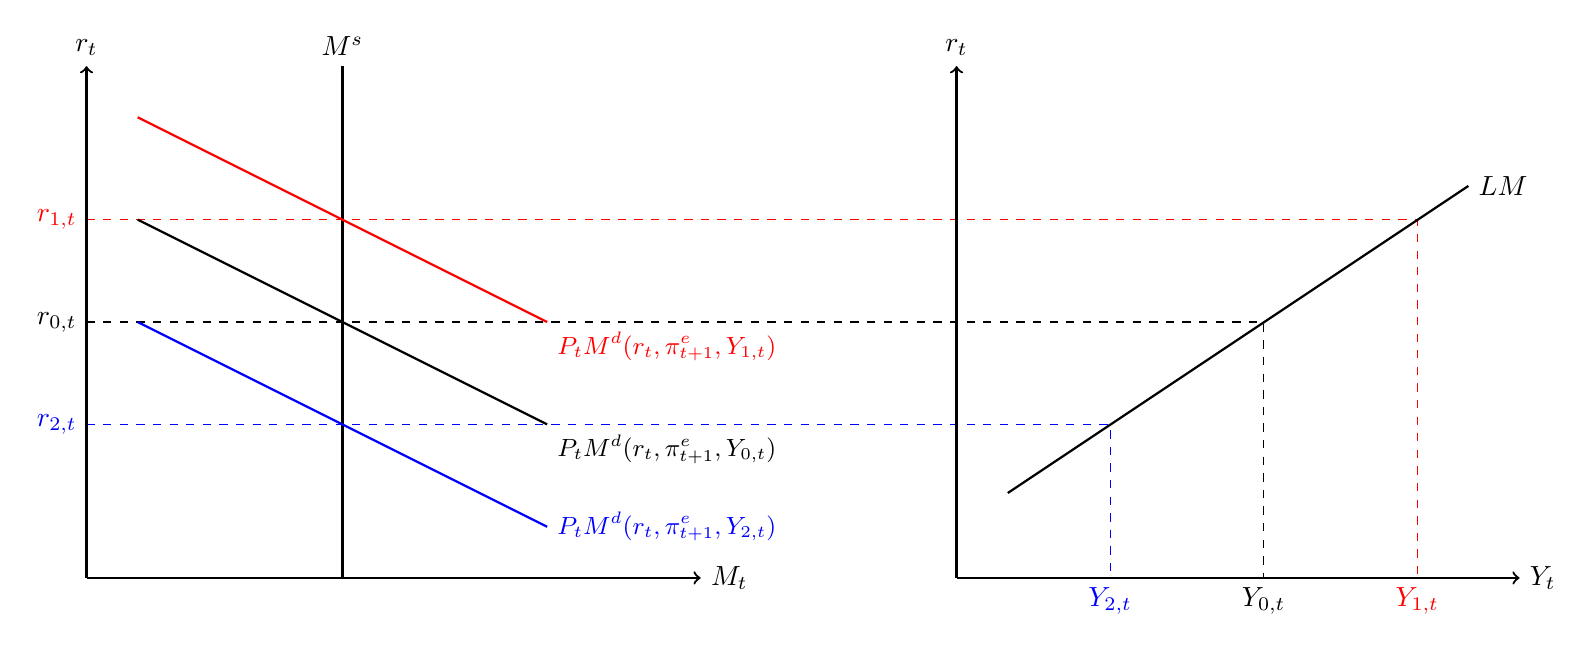
\begin{tikzpicture}[scale=1.3]

    % ==========================================
    % CONNECTING DASHED LINES (Drawn first to stay in background)
    % ==========================================
    
    % High interest rate (r1) -> High output (Y1)
    \draw[dashed, red] (0, 3.5) -- (13, 3.5) -- (13, 0);
    
    % Equilibrium interest rate (r0) -> Medium output (Y0)
    \draw[dashed, black] (0, 2.5) -- (11.5, 2.5) -- (11.5, 0);
    
    % Low interest rate (r2) -> Low output (Y2)
    \draw[dashed, blue] (0, 1.5) -- (10, 1.5) -- (10, 0);

    % ==========================================
    % LEFT GRAPH: Money Market
    % ==========================================
    
    % Axes
    \draw[thick, ->] (0,0) -- (6,0) node[right] {$M_t$};
    \draw[thick, ->] (0,0) -- (0,5) node[above] {$r_t$};

    % Money Supply (M^s) vertical line
    \draw[thick] (2.5, 0) -- (2.5, 5) node[above] {$M^s$};

    % Money Demand Curves
    % Red (Highest income Y_1)
    \draw[thick, red] (0.5, 4.5) -- (4.5, 2.5) node[below right, font=\small] {$P_t M^d(r_t, \pi_{t+1}^e, Y_{1,t})$};
    
    % Black (Middle income Y_0)
    \draw[thick, black] (0.5, 3.5) -- (4.5, 1.5) node[below right, font=\small] {$P_t M^d(r_t, \pi_{t+1}^e, Y_{0,t})$};
    
    % Blue (Lowest income Y_2)
    \draw[thick, blue] (0.5, 2.5) -- (4.5, 0.5) node[right, font=\small] {$P_t M^d(r_t, \pi_{t+1}^e, Y_{2,t})$};

    % Y-axis Labels
    \node[left, red] at (0, 3.5) {$r_{1,t}$};
    \node[left, black] at (0, 2.5) {$r_{0,t}$};
    \node[left, blue] at (0, 1.5) {$r_{2,t}$};

    % ==========================================
    % RIGHT GRAPH: LM Curve Derivation
    % ==========================================
    
    % Shift coordinate system right by 8.5cm for the right graph
    \begin{scope}[xshift=8.5cm]
        % Axes
        \draw[thick, ->] (0,0) -- (5.5,0) node[right] {$Y_t$};
        \draw[thick, ->] (0,0) -- (0,5) node[above] {$r_t$};

        % LM Curve 
        \draw[thick] (0.5, 0.83) -- (5, 3.83) node[right] {$LM$};

        % X-axis Labels
        \node[below, blue] at (1.5, 0) {$Y_{2,t}$};
        \node[below, black] at (3.0, 0) {$Y_{0,t}$};
        \node[below, red] at (4.5, 0) {$Y_{1,t}$};
    \end{scope}

\end{tikzpicture}
\end{document}
    }
\end{figure}
\begin{itemize}
\item and the AD curve.
\end{itemize}
\begin{figure}[h]
    \centering
    \resizebox{0.4\textwidth}{!}{
    \documentclass[border=10pt]{standalone}
\usepackage{tikz}
\usepackage{xcolor}
\usepackage{amsmath}

\begin{document}
\begin{tikzpicture}[scale=1.3]

    % ==========================================
    % BACKGROUND DASHED LINES
    % Drawn first so they appear behind the curves and axes
    % ==========================================
    
    % Blue (P2, Y2)
    \draw[dashed, blue] (1.5, 3.0) -- (1.5, 9.6);
    \draw[dashed, blue] (0, 3.0) node[left] {$P_{2,t}$} -- (1.5, 3.0);
    
    % Black (P0, Y0)
    \draw[dashed, black] (3.0, 2.0) -- (3.0, 8.7);
    \draw[dashed, black] (0, 2.0) node[left] {$P_{0,t}$} -- (3.0, 2.0);
    
    % Red (P1, Y1)
    \draw[dashed, red] (4.5, 1.0) -- (4.5, 7.8);
    \draw[dashed, red] (0, 1.0) node[left] {$P_{1,t}$} -- (4.5, 1.0);

    % X-axis Labels for Bottom Graph
    %\node[below, blue] at (1.5, 0) {$Y_{2,t}$};
    %\node[below, black] at (3.0, 0) {$Y_{0,t}$};
    %\node[below, red] at (4.5, 0) {$Y_{1,t}$};

    % ==========================================
    % BOTTOM GRAPH: AD Derivation
    % ==========================================
    
    % Axes
    \draw[thick, ->] (0,0) -- (6.5,0) node[right] {$Y_t$};
    \draw[thick, ->] (0,0) -- (0,4.5) node[above] {$P_t$};

    % AD Curve
    \draw[thick] (0.5, 3.66) -- (5.5, 0.33) node[right] {$AD$};

    % ==========================================
    % TOP GRAPH: IS-LM Model
    % ==========================================
    
    % Shift coordinate system up by 6cm for the top graph
    \begin{scope}[yshift=6cm]
        % Axes
        \draw[thick, ->] (0,0) -- (6.5,0) node[right] {$Y_t$};
        \draw[thick, ->] (0,0) -- (0,5.5) node[above] {$r_t$};

        % IS Curve
        \draw[thick] (0.5, 4.2) -- (6.0, 0.9) node[right] {$IS$};

        % LM Curves
        % Blue (LM(P_2,t)) - High price level
        \draw[thick, blue] (0, 2.4) -- (3.5, 5.2) node[right] {$LM(P_{2,t})$};
        
        % Black (LM(P_0,t)) - Equilibrium price level
        \draw[thick, black] (0.5, 0.7) -- (5.0, 4.3) node[right] {$LM(P_{0,t})$};
        
        % Red (LM(P_1,t)) - Low price level
        \draw[thick, red] (2.25, 0.0) -- (6.0, 3.0) node[right] {$LM(P_{1,t})$};
    \end{scope}

\end{tikzpicture}
\end{document}
    }
\end{figure}
\newpage
\begin{itemize}
\item The classical dichotomy: the real variables in the supply side ($w_t, N_t$, etc.) are unaffected by changes in the money supply or price levels.
\item Putting everything together:
\begin{figure}[h]
    \centering
    \resizebox{0.8\textwidth}{!}{
    \documentclass{standalone}
\usepackage{tikz}
\usepackage{amsmath}

\begin{document}

\begin{tikzpicture}[xscale=1.0, yscale=1.0, >=stealth]
% --- Global Styles ---
\tikzstyle{axis} = [->, thick]
\tikzstyle{curve} = [thick]
\tikzstyle{dashline} = [dashed, thick]

% --- Panel Origin Coordinates ---
\def\xl{0}    % Left column X-coordinate
\def\xr{8.5}  % Right column X-coordinate
\def\yt{14}   % Top row Y-coordinate
\def\ym{7}    % Middle row Y-coordinate
\def\yb{0}    % Bottom row Y-coordinate

% --- Key Alignment Offsets ---
\def\n0{3.5}     % N_{0,t} intersection offset
\def\yp0{3.2}    % Y_{0,t} intersection offset
\def\w0{2.5}     % w_{0,t} intersection offset
\def\p0{2.5}     % P_{0,t} intersection offset
\def\r0{2.5}     % r_{0,t} intersection offset

% ==========================================
% BOTTOM LEFT: Production Function
% ==========================================
\draw[axis] (\xl, \yb) -- (\xl+6, \yb) node[right] {$N_t$};
\draw[axis] (\xl, \yb) -- (\xl, \yb+5) node[above] {$Y_t$};

% Production Curve
\draw[curve] (\xl, \yb) to[out=70, in=195] (\xl+\n0, \yb+\yp0) to[out=15, in=180] (\xl+5.5, \yb+3.6) node[right] {$A_t F(K_t, N_t)$};

% Point projections & labels
\draw[dashline] (\xl+\n0, \yb) node[below] {$N_{0,t}$} -- (\xl+\n0, \yb+\yp0);
\draw[dashline] (\xl, \yb+\yp0) node[left] {$Y_{0,t}$} -- (\xl+\n0, \yb+\yp0);

% Horizontal dashed line spanning the gap to the reflection panel
\draw[dashline] (\xl+\n0, \yb+\yp0) -- (\xr+\yp0, \yb+\yp0);


% ==========================================
% MIDDLE LEFT: Labor Market
% ==========================================
\draw[axis] (\xl, \ym) -- (\xl+6, \ym) node[right] {$N_t$};
\draw[axis] (\xl, \ym) -- (\xl, \ym+5) node[above] {$w_t$};

% Labor Supply and Demand Curves (Centered strictly on intersection)
\draw[curve] (\xl+\n0-2.5, \ym+\w0-2) -- (\xl+\n0+2.5, \ym+\w0+2) node[right] {$N^s(w_t, \theta_t)$}; 
\draw[curve] (\xl+\n0-2.5, \ym+\w0+2) -- (\xl+\n0+2.5, \ym+\w0-2) node[right] {$N^d(w_t, A_t, K_t)$}; 

% Point projections & labels
\draw[dashline] (\xl+\n0, \ym+\w0) -- (\xl, \ym+\w0) node[left] {$w_{0,t}$};

% Vertical dashed line dropping down to the production function
\draw[dashline] (\xl+\n0, \ym+\w0) -- (\xl+\n0, \yb+\yp0);


% ==========================================
% BOTTOM RIGHT: Reflection Panel
% ==========================================
\draw[axis] (\xr, \yb) -- (\xr+6, \yb) node[right] {$Y_t$};
\draw[axis] (\xr, \yb) -- (\xr, \yb+5) node[above] {$Y_t$};

% 45-degree reflection line
\draw[curve] (\xr, \yb) -- (\xr+4.5, \yb+4.5) node[right] {$Y_t = Y_t$};

% Point projections & labels
\draw[dashline] (\xr+\yp0, \yb+\yp0) -- (\xr+\yp0, \yb) node[below] {$Y_{0,t}$};

% Vertical dashed line going up to the AS-AD panel
\draw[dashline] (\xr+\yp0, \yb+\yp0) -- (\xr+\yp0, \ym);


% ==========================================
% MIDDLE RIGHT: AS-AD Model
% ==========================================
\draw[axis] (\xr, \ym) -- (\xr+6, \ym) node[right] {$Y_t$};
\draw[axis] (\xr, \ym) -- (\xr, \ym+5) node[above] {$P_t$};

% AS Curve (Vertical at Y_{0,t})
\draw[curve] (\xr+\yp0, \ym) -- (\xr+\yp0, \ym+4.5) node[above right] {$AS$};

% AD Curve (Centered strictly on intersection)
\draw[curve] (\xr+\yp0-2.2, \ym+\p0+1.8) -- (\xr+\yp0+2.2, \ym+\p0-1.8) node[right] {$AD$}; 

% Point projections & labels
\draw[dashline] (\xr+\yp0, \ym+\p0) -- (\xr, \ym+\p0) node[left] {$P_{0,t}$};

% Vertical dashed line continuing up to IS-LM
\draw[dashline] (\xr+\yp0, \ym+4.5) -- (\xr+\yp0, \yt);


% ==========================================
% TOP RIGHT: IS-LM Model
% ==========================================
\draw[axis] (\xr, \yt) -- (\xr+6, \yt) node[right] {$Y_t$};
\draw[axis] (\xr, \yt) -- (\xr, \yt+5) node[above] {$r_t$};

% IS Curve (Fixed and centered strictly on Y_{0,t} intersection)
\draw[curve] (\xr+\yp0-2.2, \yt+\r0+2.2) -- (\xr+\yp0+2.2, \yt+\r0-2.2) node[right] {$IS$}; 

% LM Curve (Fixed and centered strictly on Y_{0,t} intersection)
\draw[curve] (\xr+\yp0-2.2, \yt+\r0-2.2) -- (\xr+\yp0+2.2, \yt+\r0+2.2) node[right] {$LM$}; 

% Point projections & labels
\draw[dashline] (\xr+\yp0, \yt+\r0) -- (\xr, \yt+\r0) node[left] {$r_{0,t}$};
\draw[dashline] (\xr+\yp0, \yt) -- (\xr+\yp0, \yt+\r0);

\end{tikzpicture}

\end{document}
    }
\end{figure}
\item Here, we can see that changes in $Y_t$ must be driven by supply-side shocks, as $Y_t$ is fixed by the vertical AS curve.
\end{itemize}


\begin{itemize}
\item A New Keynesian model makes use of a partial sticky price setting to the AS curve:
\[
P_t = \bar{P}_t + \gamma(Y_t - Y^f_t)
\]
\item Therefore,
\end{itemize}
\newpage
\begin{figure}[h]
    \centering
    \resizebox{0.75\textwidth}{!}{
    \input{newkeynesian}
    }
\end{figure}

\begin{itemize}
\item Note that the full-employment AS curve, $AS^f$, is hypothetical here, and movements should occur along the upward-sloping AS curve.
\item In this model, demand-side shocks usually cause inefficiency in the labor market.
\item Again, examples of movements are omitted, but it is worth analyzing the effects of different shocks and fiscal / monetary policies.
\item What if the central bank directly controls $r_t$?
\[
r_t = r({(\ln Y_t - \ln Y_t^f})^+, P_t^+)
\]
\item Recall that:
\[
\frac{M_t}{P_t} = C_t^{\frac{\sigma}{v}}\left(\frac{1+r_t+\pi^e_{t+1}}{r_t + \pi^e_{t+1}}\right)^\frac1v
\]
\item Then the LM curve is still upward-sloping, but $M^s = \frac{M_t}{P_t}$ is now endogenous.
\end{itemize}

\end{document}

